
\chapter{Discussion}
\label{Conclusions}
\section{Conclusions}

\paragraph{L'objectif de ce travail} a été de vérifier\textbf{ l'hypothèse du caractère
révélateur du test
d'écoute }de Tomatis \textbf{ sur l'impact du processus musicothérapeutique},
et, d'autre part, à s'ouvrir à d'autres
domaines d'exploration.

Les interrogations au début de notre parcours au
sujet de la carence d'outils d'évaluation objective, se
reformulent comme suit:
\begin{itemize}
     \item
     %  La quantification d'écoute par un test  aboutirait-elle à une
      % transformation, en d'autres mots, une constatation de transformation serait-elle relevable
       %par la quantification d'un test.
       Si l'écoute est quantifiable  par un test, pourrait-on assister à sa
transformation?
\item Si cette transformation existe, serait-elle reliable avec
une prise en charge musicothérapeutique?
\item Cette transformation de l'écoute aurait-elle un impact sur l'état
psychique du patient? %source principale de notre intérêt.
\end{itemize}
% bibliographie + réf. chapitre partie théorique!!!!



  Compte tenu de la multiplicité quantitative et qualitative des
  résultats, notre intérêt s'est centré essentiellement sur l'\textbf{analyse d'une
  observation}, portant \textbf{sur la transformation de l'écoute} à l'aide de
  l'appareil test, utilisable par ailleurs, comme outil complémentaire
  et porteur d'indications pré/post-thérapie.

  Avec toute la
  complexité des aspects audiologiques et psychologiques,
  et suite aux comparaisons
  pré/post-thérapie introduites spécifiquement sur les 30 tests d'écoute et 9 questionnaires WQ, nous
  avons relevé des \textbf{transformations d'écoute
   individuelles et
  catégorielles importantes pour le groupe de musicothérapie} alors que
  la différence est bien moins notable dans le groupe contrôle.



  \textbf{Groupe Contrôle:} 	          \textbf{ test d'écoute: ``=''   et    WQ: ``-'}


  \textbf{Groupe Musicothérapie:}     \textbf{test d'écoute: ``+''      et    WQ: ``+''}



  Ainsi, pour répondre aux hypothèses formulées:
  \begin{itemize}
       \item
          L'écoute est quantifiable  par un test, nous avons pu l'observer et   assister à sa
  transformation.

  \item Cette transformation peut être reliée  avec
  une prise en charge musicothérapeutique, puisque nous avons pu constater une différence entre les deux groupes, le GM et le GC.

  \item Cette transformation de l'écoute a eu  un impact sur l'état
  psychique du patient, source principale de notre intérêt, la corrélation étant claire entre le test d'écoute et le questionnaire.
  \end{itemize}

  \textbf{ En conclusion, le test
  d'écoute peut être considéré comme une source de données
   intéressantes et/ ou complémentaires, pouvant par conséquent, être
  \textbf{révélateur d'un
  travail en musicothérapie}}.





\section{Considérations sur les séances de musicothérapie}
              Lors de leur déroulement, les séances de
              musicothérapie n'ont pas été
décortiquées pour analyser leur impact. C'eût
été passionnant de le faire mais ici, ce n'était pas notre objectif.


Par contre, nous avons fait quelques rapprochements intéressants dans les perspectives d'une analyse plus
poussée et plus importante pour laquelle nous avons  relié\textbf{ les trois zones du
test d'écoute avec des données musicothérapeutiques.}
(Cf. Fig. 5. 1).
Nous avons aussi mis
en parallèle  l'utilisation d'instruments,(Cf. Annexe, Fig. C.1.)
indicateur éventuel des zones de fréquences à
privilégier.
%Chaque instrument a une tessiture
%différente avec une plage
%définie de fréquences. Selon l'analyse de l'écoute du patient, le choix
%d'instrument à privilégier sera plus rapide et plus sûr.

\begin{figure}[tbh]
	\centering
	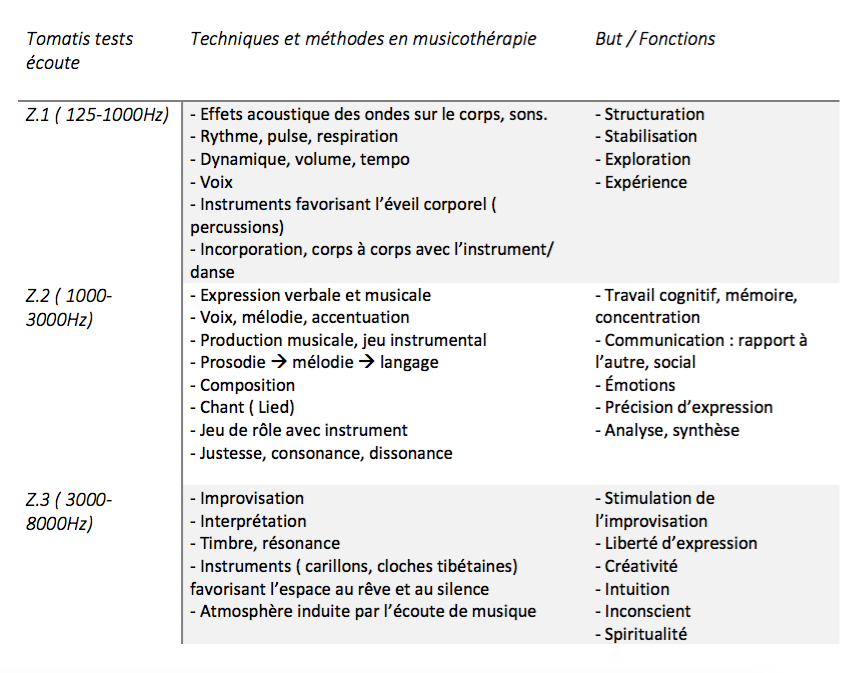
\includegraphics[width=1\linewidth]{images/testtechnmethbut}
	\caption[Zones du test avec la musicothérapie]{Les 3
          zones et la musicothérapie}

	\label{testbutetfonction}
\end{figure}



En complément, nous allons décrire avec un patient le déroulement de deux séances de
musicothérapie accompagnée uniquement de leur test d'écoute, de
manière totalement indépendante car, nous en avons conscience, pas
suffisament représentative.

\subsection{Patient M:}

%Données amnamestiques: âge, profession, famille etc., raison d'hospitalisation
\textbf{ Test d'écoute pré -- musicothérapie:}
 	Le patient est venu en clinique en raison d'un burnout. Il se montre très
        intéressé pour participer à l'étude. Nous allons faire
        l'observation plus attentive de
        son oreille droite, (Fig.4.22), l'oreille ``directrice'',
        celle qui est la plus perturbée dans son cas.


 	\begin{figure}[tbh]
 		\centering
 		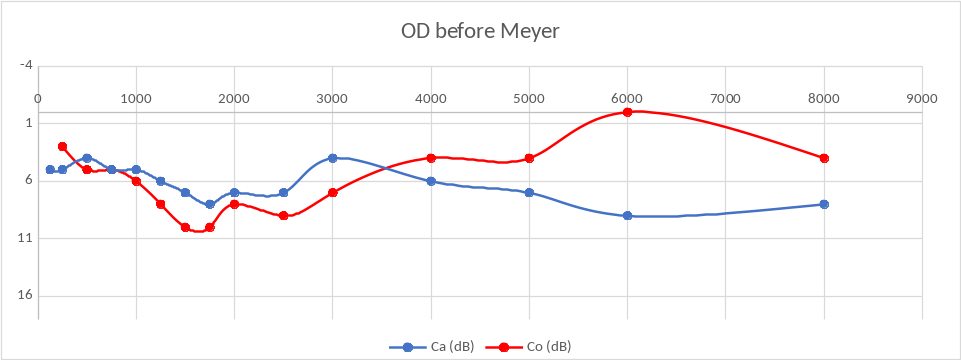
\includegraphics[width=0.7\linewidth]{images/clinique/od_before_meyer.png}
 		\caption{Test d'écoute avant musicothérapie}
 		\label{fig:odbeforemeyer}
 	\end{figure}


   	\begin{figure}
   		\centering
   		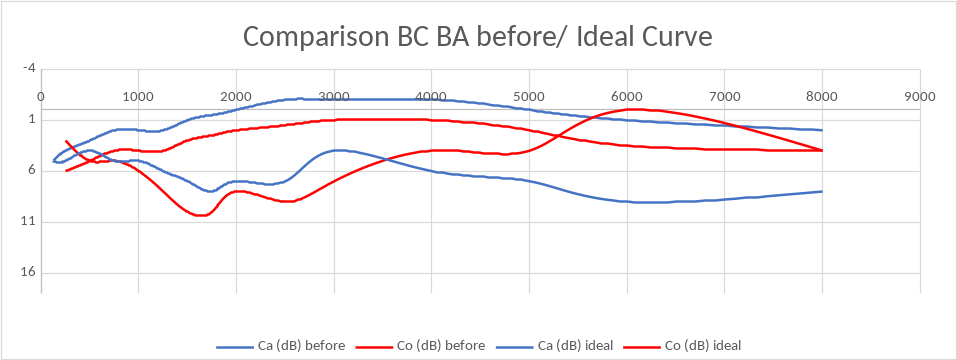
\includegraphics[width=0.7\linewidth]{images/clinique/comparison_bc_ba_before_vs_ideal_curve_meyer.png}
   		\caption[Comparaison avec la courbe idéale]{Comparaison avant
                    musicothérapie des
                    courbes  avec la courbe idéale}
   		\label{fig:comparisonbcbabeforevsidealcurvemeyer}
   	\end{figure}


     	 \textbf{Déroulement général} :
    Ayant le choix devant un grand instrumentarium,
            le patient se dirige spontanément vers le piano, et très vite
            l'\textit{émotion} monte: il pense à son père qui en jouait et qui
            s'énervait contre lui, enfant essayant d'en
            jouer. Il n'a jamais pris de cours, tapote avec un seul doigt et \textit{se considère comme
            amusica}l. Il essaie ensuite l'orgue électrique: les \textit{sons bas}
            lui procurent un énorme plaisir mais il n'ose pas enfoncer les touches
            complètement car c'est trop fort, dit-il; d'autre part, il
            craint également les
            \textit{sons hauts.}
            Après un moment,la thérapeute lui suggère d'essayer avec deux doigts.
            Il enclenche le mode ``choeur'' et les sons se font beaucoup
            plus présents, plus forts, mais il les accepte. Puis il commence à essayer spontanément
            avec les autres doigts et remarque en s'étonnant qu'il se
            dirige tout de même vers les sons
            hauts. Il \textit{s'amuse} à mêler les différentes tessitures,
            le haut comme le bas.
            Il enclenche le mode ``drums'' et part d'un\textit{ joyeux
            fou-rire}. Retour en enfance, dit-il.
            Il \textit{se détend} et prend de plus en plus de plaisir à jouer, particulièrement  les sons élevés
            sur la droite et avec la main droite, et fait
            la remarque suivante très surprenante:
            \textit{``Ich kann meine Gefühle mit der rechten Hand steuern!''
            ``Je peux diriger mes sentiments avec ma main droite''.}
     Son expression à ce moment précis de la séance est saisissante: il
            est gaucher et se sent très à l'aise d'utiliser son autre
            main,-- \textit{``Komisch''},  \textit{``Etrange''}, se fait-il
            en réflexion, très surpris de sa réaction-- et c'est un événement
            accueilli comme une vraie
            découverte--\textit{``Entdeckung''} --.
            Il ajoute de plus, très affirmatif, que les sentiments avec sa main
            droite ne sont plus une affaire de tête. \textit{``Keine
            Kopfsache mehr'''}. Il veut expérimenter le contraire, fait
          une inversion d'utilisation des mains pour s'en convaincre et tout redevient comme
            avant, c.à.dire \textbf{non fluide et retour au contrôle
              mental},
            ``bloquant'', dit-il. En inversant à nouveau, il retrouve
            détente et fluidité.
            A la séance suivante, il aimerait pouvoir ressentir
            les sons dans tout son corps et ce sont les\textit{ bols
              tibétains } qui lui
            apporteront tranquilisation et
            énergie. Utiliser désormais sa main
            droite avec confiance l'aide, à ses dires, à analyser les
            situations dans lesquelles il se trouve.
            Nous avons mis quelques mots en italique soulignant des  points
            importants qu'amè\-ne un suivi en musicothérapie: l'émotion qui surgit très
            vite,
            l'attention du patient complètement happé par les sons --qui l'a
            contraint à être dans "l'instant présent "" ou une forme de méditation, la joie
            enfantine qui réémerge avec le rire, la détente et la découverte,
            ses propres observations et réflexions.
            Il y a une imbrication forte des cinq sens, accompagnée par l'émotionnel, le comportemental, la
            mémoire, en bref tout le système limbique et l'aspect
            physiologique et psychologique.

            De manière plus précise, nous faisons le constat, dans ce cas
            particulier,  de la relation main droite, oreille droite, écoute
            à droite et du probable impact sur l'hémisphère gauche.
            Evidemment, nous ne pouvons généraliser son cas, (peut-être dû au hasard ou aux circonstances) et n'émettre qu'une hypothèse
            en mettant en relation la nécessité d'une stimulation au niveau du cortex préfrontal
            gauche -- partie de l'hémisphère gauche que l'écoute avec
            l'oreille droite inciterait (génèrerait) -- pour activer l'analyse et la
            mise en perspective des situations. Le but étant de trouver ou
            retrouver un équilibre, une forme d'harmonie ou d'homéostasie, ce qui corroborerait les
            propos de T. Janssen (T. Janssen, 191)  démontrant la gestion des émotions par
            l'un et l'autre des 2 hémisphères, soit le droit,  gérant les désagréables
            (réflexe de survie, ne devant néanmoins pas se prolonger au risque de
            développement de pathologies)
            et l'autre, le gauche --- plus récent en terme d'évolution ---  les
            agréables, indispensables pour relativiser       les situations.


            \textbf{ Test d'écoute post -- musicothérapie:}



             	\begin{figure}[h]
             		\centering

             		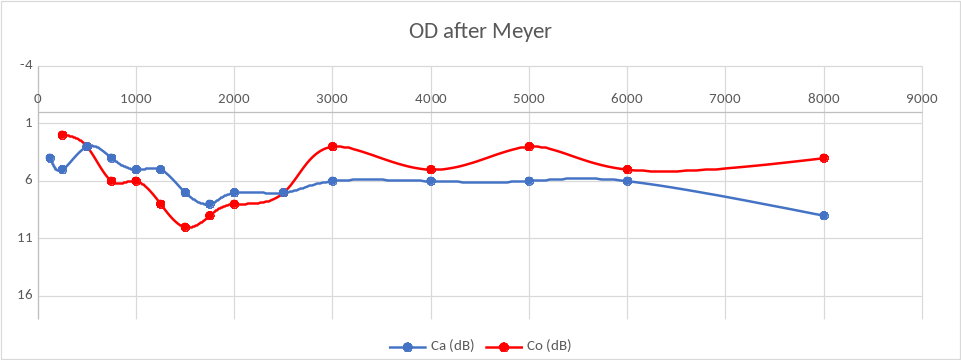
\includegraphics[width=0.7\linewidth]{images/clinique/od_after_meyer.png}
             		\caption{Test d'écoute après la musicothérapie}
             		\label{fig:odaftermeyer}
             	\end{figure}
             Les figures 5. 2  5. 3 et 5. 4 correspondent à l'oreille droite.
                    Nous faisons les observations suivantes:
                  Dans les
                    zones 2 et 3,  la courbe aérienne s'est modifiée, freinant sa
                    chute et se stabilisant à l'horizontal entre 3000 et 6000 Hz
                    avec des seuils de 5/6= 25 dB.
                    Dans les mêmes zones 2 et 3, la
                    courbe osseuse montait de 2500 à 6000 mais après traitement,
                    elle se modifie, se rapproche et abaisse ses seuils de
                    sensibilité en étant moins réactive aux sons de faible
                    intensité, donnée très positive: ainsi le très grand écart visuel dans la zone 3 s'amenuise beaucoup. Au niveau de cette
                    zone, une large progression dans
              le domaine de la créativité semble s'élaborer.Avec les
                seuils
                 de c.aérienne et c.osseuse des\textbf{ deux} oreilles (\textbf{droite et gauche)} en prenant
                 référence la courbe idéale, nous
                constatons par contre les modifications suivantes pré/post-traitement:
                c.a.: 6,43/6,03 et c.o.: 6,25/6,85.
                Ces chiffres se sont nettement
                modifiés et tendent vers
                ceux dits ``idéaux''  qui équivalent aux environs de 1,3 pour
                c.a. et 3,1 pour c.o. L'écart reste cependant très important. % A
                %des dégâts subis aux oreilles,dus aux  détonations d'armes manipulées en sa présence et
                % sans protection, selon les dires du patient.
                Et, de plus, en observant la moyenne de son oreille gauche et droite pré/post-traitement,
                (Cf. Fig. 4. 14 et 4. 15, Patient M. groupe GM), le
                nombre de croisements n'a ni augmenté ni diminué, ce qui nous donne
                aucun élément constructif.

                En résumé, son écoute générale est très mobile, elle bouge avec un
                net profil d'amélioration, et plus particulièrement avec l'oreille
                droite comme évoqué plus haut. L'ensemble est positif, tend vers un
                rééquilibrage. Le recueil des données du
                questionnaire WHOQOL l'atteste et le confirme.
                Il reste cependant encore de larges perspectives de travail et d'amélioration.
                Par conséquent, le test d'écoute est susceptible d'apporter des renseignements, lors
                    d'une analyse succinte pré/post-traitement.






                    \section{Considérations complémentaires:}


                  \textbf{Les troubles de l'humeur et leur expression
                  musico-phy\-sico-psy\-cho\-lo\-gi\-que:}
                  D'une manière plus générale, par le lien entre les troubles
                  émotionnels et le
                  système sensoriel, notamment avec le cortex auditif, nous
                  pouvons dresser un portrait
                  physico-psychologique de ce type de population,
                  en les mettant en correspondance avec les zones du test d'écoute et
                  en y ajoutant quelques remarques sur les modifications vocales.

                  \textbf{Un test représentatif}:
                  Dans l'illustration ci-dessous représentant un test
                  d'écoute d'un sujet atteint de dépression, la
                  chute dans les zones de fréquences élevées est
                  clairement visible. Elle correspond au rapport de l'émission du son à
                  très faible intensité en rapport avec
                  l'instant perçu par le
                  patient, autrement dit  -- à une augmentation
                  du volume
                  par le thérapeute jusqu'à ce que le patient les entende et les signale
                  --- .
                  Ce sont ses seuils minima de fréquences.
                  \begin{figure}[ht]
                  \centering
                  \includegraphics[width=0.7\linewidth]{images/courbesdeepressif.jpg}
                  \caption{Courbes particulières d'un sujet diagnostiqué dépressif}
                  \label{fig:courbes du dépressif}
                    \end{figure}


                          \paragraph{Descriptif selon les zones d'nterprétation:}

                    \begin{itemize}
                      	\item Zone 1 :  Le rythme cardiaque: un stress intense va modifier le rythme
                      du corps en augmentant ses fréquences. La respiration deviendra
                      rapide. Il va s'en suivre une modification des perceptions
                      extérieures. Une sensibilité particulièrement accrue aux bruits et
                      aux sons peut en découler et être vécue comme une
                      atteinte physique et psychique insupportable.
                      Le changement de posture et d'attitude corporelle sont
                    notables (affaissement) et la perte d'énergie physique considérable (épuisement).
                    	\item Zone 2: La qualité de la voix: changement de la qualité du timbre de la
                     voix et de l'émission verbale.
                      La voix se caractérise par son volume, son timbre, sa mélodie et son
                      langage. Nous pouvons en faire le
                            descriptif général, rejoignant ainsi l'idée émise lors du Congrès de la Société
                            américaine d'acoustique \autocite{le_service_metronews}
                            %https://www.lci.fr/sante/et-si-on-diagnostiquait-la-depression-avec-u
                            %n-test-vocal-sur-smartphone-1562728.html,
                            de diagnostiquer la
                            dépression par la voix:\footnote{Maryland University, 2004, 168\ieme\ Congrès de la Société
                    américaine d'acoustique.}

                     	\begin{enumerate}
                     		\item le volume : basse intensité, faible dynamique
                     		\item la mélodie : monotone, sans modulation
                     		\item le timbre : mauvaise qualité due à une pertes des harmoniques
                     		\item le langage : difficulté d'élocution, manque de fluidité
                     	\end{enumerate}
                            Il en découle une communication difficile avec l'entourage qui
                            conduit au retrait social et à l'enfermement sur soi.

                            De même, un analyseur vocal peut permettre de suivre précisément l'amélioration de
                            l'identité vocale; sa visualisation conforte les progrès grâce aux
                            formants. L'enveloppe spectrale montre le timbre plus ou moins riche
                            dans l'empreinte vocale, renseignements précieux selon les cas.

                            	\item Zone 3: La confusion mentale, la démotivation, la perte d'énergie
                            psychique, la disharmonie intérieure/extérieure, le non-verbal.
                            \end{itemize}



                             % \begin{figure}
                            %	\centering
                            %	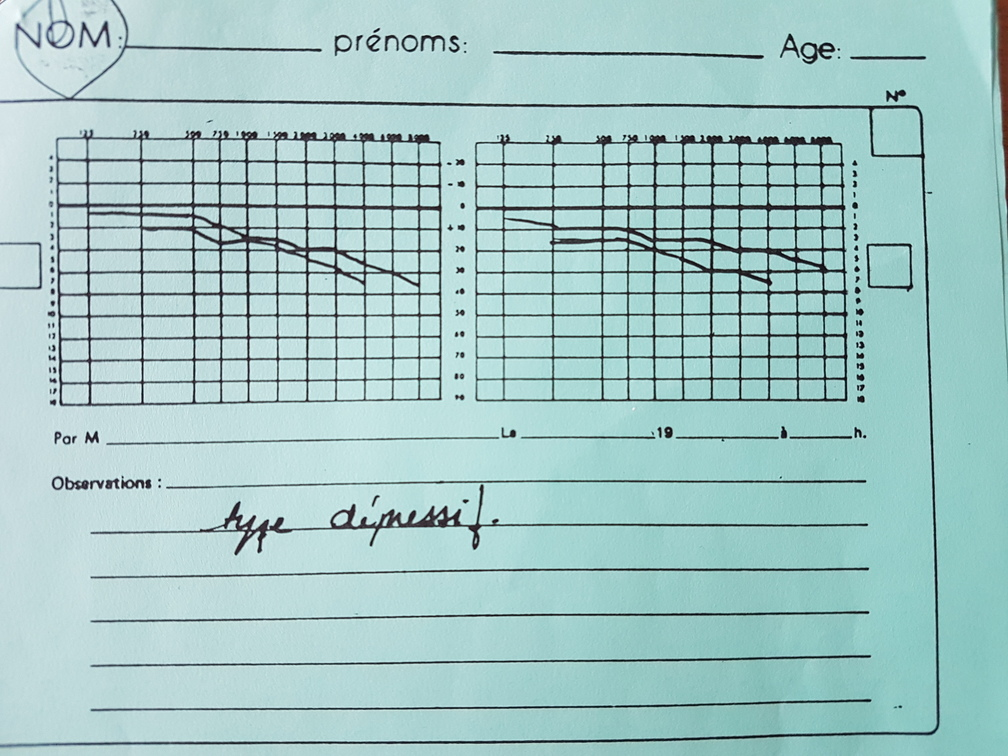
\includegraphics[width=0.7\linewidth]{images/courbedepressif.jpg}
                            %	\caption[Exemple d'une courbe de dépressif]{Courbe
                             %         représentative d'un dépressif, extrait de l'étude de Nantes,
                               %      1987.}

                            %	\label{groupecontroleimage1}
                            %\end{figure}


                            	\textbf{Résonance des informations récoltées par les 3
                                      zones du test d'écoute en musicothérapie et en
                              psychologie :}

                            \begin{itemize}
                             \item  Z.1: le physique, le corps, l'incorporation et
                            l'intégration du rythme,
                            la posture d'écoute  =  Rythme, tempo, puls

                            \item  Z.2:  l'expression vocale, la communication,
                            l'émotionnel, la sensibilité, l'affect = Voix, timbre, mélodie

                            \item Z.3: la créativité, l'interprétation, la
                            résonance, la musicalité, la motivation, le non-verbal (l'intraduisible en mot), l'espace = Justesse, harmonie (consonance,
                            dissonance), improvisation.
                            %\footnote{\{Hegi : L'improvisation joue un rôle centrale en musicothérapie (Hegi 1986)}
                            \end{itemize}

                            Pour une optimalisation de l'écoute différenciée, il est souhaitable
                            de rejoindre dans un premier temps  le patient dans sa capacité
                            d'écoute de base, avec une adaptation et modulation consécutive du
                            volume sonore (seuils auditifs) et de l'utilisation de la voix (zone
                            2) en musicothérapie.
                            L'existence de difficultés de perception dans cette zone nous
                            induit à une meilleure compréhension et  élucidation de ces dernières à l'aide du
                            test d'écoute.

                            Pour élargir le concept de\textbf{ la zone 3,} comme on le
                            verra dans la rubrique des réflexions, nous pourrions
                            également l'étendre aux notions winnicottiennes du jeu, de la capacité
                            créative dans un espace
                            intermédiaire, où l' \textit{``objet
                            transitionnel'' } de D. Winnicott dans \textit{``Jeu et Réalité''}
                            \autocite{winnicott}
                            figure entre le ``le
                            dedans et le
                            dehors'',
                            l'interne et l'externe, et de là,  prolonger le questionnement du
                            rapport avec le concept des
                            courbes aérienne et osseuse.



                            Si on considère que ``\emph{l'alliage indissociable du corps et du psychisme,
                            visible et lisible résulte de l'écoute de
                            sons'''}\footnote{\emph{Extrait de l'entretien Tomatis réalisé par
                              Auriol, Anvers 1973}}, le concept de dépression (R. Jouvent) \autocite{doronparot} (Cf. Annexes
                            A.5) inclut aussi l'idée d'une protection et une stratégie de
                            défense du psychisme, ayant un lien évident avec les zones du schéma d'écoute.

                            Même chez E. Willems \autocite{willems} \footnote{\textit{Philosophie de la méthode} issu de sa
                            Pédagogie musicale, Copyright by Musique et Culture, Strasbourg}, on relève des correspondances analogues entre les vies
                            corporelle (impulsions physiques)
                            --- rythmique, affective (affection et sentiment) --- mélodique, mentale
                            (raisonnement et intellect) --- harmonique.


                            De plus, si nous nous référons à la conception indienne antique des chakras
                            ainsi qu'au sens de la seconde
                            topique de Freud (\textit{ça, moi et surmoi}), nous trouvons également des correspondances
                            entre les trois zones de
                            fréquences et \textit       {``la distribution de l'énergie pulsionnelle''} ou entre
                            les
                            \textit{``caractéristiques du son et l'énergie
                            instinctuelles''}\autocite[ch. 13]{auriol_cle_1996}.

                            \begin{figure}
                            	\centering
                            	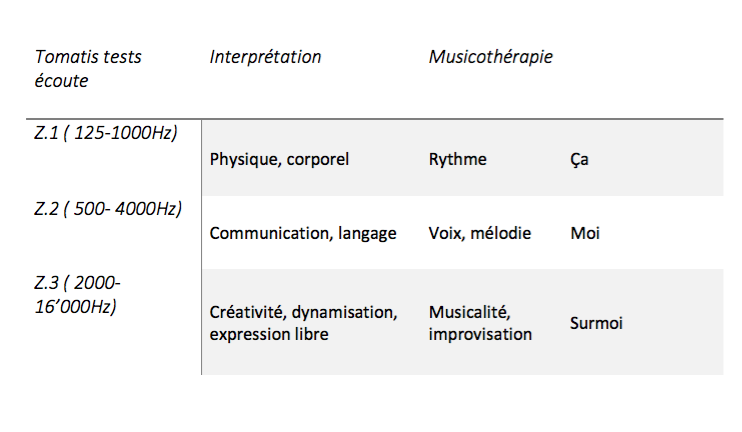
\includegraphics[width=1.0\linewidth]{images/testinterpmusico}
                            	\caption[ L'interprétation des 3 zones et leur correspondance
                                    en musicothérapie]{Graphique: interprétation des 3 zones du
                                      test, leur correspondance en musicothérapie et selon les
                                      topiques de Freud.}

                            	\label{graphiquecolonnetestmusico}
                                  \end{figure}




                            %`\textit{`La mélodie est la seule forme musicale de la décharge individuelle,
                            %car le rythme est le moteur, pré-musical, et l'harmonie,
                            %supra-individuelle ``} (Mosonyi, 1835????, cité par Michel, 1965).


                            Ainsi, au lieu de séparer les trois grandes voies de la psychologie du
                            XXème siècle (psychanalyse, comportementalisme et pychologie
                            humaniste) comme nous le suggère T. Janssen
                            \autocite[197]{van_eersel_cerveau} il serait intéressant de les
                            considérer comme complémentaires.
                            %, comportant chacun un aspect qu'il
                            %nomme ``phénomène humain''.






\section{Mesure du test et trans\-for\-ma\-tion de l'écoute}
\textbf{Réflexions:}
L'importance de l'écoute relevée dans notre travail
%s'associe
s'allie aux nombreuses con - nexions nerveuses entre l'oreille et les
différentes parties cérébrales, incluant par la même, les aspects kinésiques
et posturaux, ainsi que toute production vocale et langagière,
dont l'ensemble en dépend.



S. Aubert -Khalfa et son équipe multidisciplinaire \autocite{affectiveDisorders} avaient déjà
exploité le test Tomatis -- sensible à la différence des
seuils auditifs -- entre une population
dépressive avec stress post-traumatique et une population normale.
D'autre part, l'importante\textbf{ sensibilité des seuils auditifs }observés chez des
sujets à dépression majeure figure aussi dans les découvertes de Yowell and Co.
\autocite{affectiveDisorders}\footnote{cité
par S.Aubert- Khalfa et al.: Yovell, Y.,
  Sackeim,H.A., Epstein, D.G.,Prudic, J., Devanand, D.P. McElhiney,
  M.C. Settembrino, J.M. Bruder, G.E., 1995. Hearing loss asymmetry in
  major depression.J.Neuropsychitr. Clin. Neurosci. 7, 82--89 / Journal of Affective Disorders 127
  (2010) 170}

Ces études figurent au fond comme un cheminement précurseur de notre
travail avec des \textbf{résultats convergeants}. Elles comportent par ailleurs certaines différences dans la
 procédure:  %dans le recueil de points communs des seuils
 % auditifs,
 en effet, nous avons choisi
 une population de même type de pathologie, séjournant en clinique (Klinik von Meiringen) --- sans
 groupe comparatif en bonne santé --- répartie en 2 groupes,
dont l'un a bénéficié de
musicothérapie.





%Nous avons utilisé un type de test d'écoute dont nous soulignons la
%complexité du test d'écoute utilisé.%, puisant
%à la fois ses racines dans l'audiologie et à la fois dans la psychologie.
%Par celui-ci, nous voyons
%qu'il  existe une possible transformation
%individuelle lors d'une
%thérapie tout
% en constatant une forme de singularité pour chacun et une
%certaine similarité selon certaines pathologies. --Comme nous l'avons
%constaté avec l'étude J.P.Granier... il existe des points communs lors des recueils des seuils
%auditifs--.

%Nos résultats
%principaux sont les suivants:

%le groupe de musicothérapie a démontré une réactivité très positive
%dans son écoute par comparaison pré/post-thérapies tandis que
%le groupe de contrôle n'a démontré qu'une très faible
%modification dans son écoute.
%Il existe ainsi une différence importante entre les résultats des
%deux groupes.

%Il convient à présent de discuter des aspects énoncés (test et
%mesures),  puis des
%limites et perspectives.
%et les résultats obtenus.


Dans l'accompagnement thérapeutique évolutif du patient,
 les transformations perceptives visibles sur
\textit{``le tracé sonore''} nous ouvrent à une modulation
musicothérapeutique mieux adaptable et différemment ajustable.
 %basée sur un test de reconnaissance de sons permettant sa

%Par comparaison, nous pouvons faire ce constat, positif ou
%négatif, ce qui est
%difficile dans la majorité des cas, nous fiant plus à notre intuition
%qu'à des données.
%Il y a une modification de l'écoute du patient lors de séances en
%musicothérapie et celle-ci est visible et lisible au moyen du test
%d'écoute employé.

%afin de l'accompagner dans son cheminement thérapeutique.

\paragraph{\textbf{Anamnèse et bilan en musicothérapie}}
Du point de vue descriptif, nous pouvons considérer un temps qui
précède
l'amorçage de la thérapie, suivi d'un temps éminemment thérapeutique.


En réalité, ces aspects s'enchevêtrent à un point tel que
l'utilisation du test peut assumer un rôle musicothérapeutique, fournissant des
  renseignements complémentaires à l'anamnèse sous forme de multiples
  aspects du son. En effet, il est  question d'émission des sons de
  l'appareil vers le patient, ainsi que sa réaction verbale et gestuelle.
En plus, l'utilisation
   du dispositif favorise une atmosphère rassurante dans la diade
   patient-thérapeute, encourageant ainsi la complicité collaborative
%ent soit abordé par une\textbf{
 % procédure de test} à l'aide d'un appareil peut être fréquemment
  % perçu comme rassurant, dans leur confusion la plus totale selon
  % certains troubles, puisque
    %jouant souvent
  %un rôle de fiabilité, de soutien.
   %et la création d'une alliance thérapeutique.
   %la présence d'un thérapeute et son alliance.
%   consiste en plusieurs rôles intrinsèques dont le travail sur le son et
% l'alliance thérapeutique.
 %Devant le flou persistant souvent sur le concept de la
%musicothérapie, il représente une forme
%d'introduction simple et claire.
 indispensable à toute
 thérapie.
Ce qui nous permet de soutenir que
 \textbf{l'alliance thérapeutique} demeure axée, comme le relève Gindl
  \autocite{gindl} sur
 un phénomène de \textbf{résonance}\footnote{Selon Doron et Parot, l'acception de ce terme se relate, d'une part, au processus psychique
primaire symbiotique entre l'enfant et sa mère et, d'autre part, à
niveau groupal où le fantasme d'un participant éveille des fantasmes chez d'autres membres du groupe en relation
de résonance  avec le premier.} \autocite{doronparot}.
%ite ``fantasmatique'' ou et aussi-- comme l'ensemble des réponses
%émotionnelles et comportementales inconscientes à la présence d'un
%autre individu-- et celle dite  ``intime'' de Rorschach avec 4 types à
%dominante kinesthésique et/ou sensorielle.
%En effet, les différentes significations
%de ce vocable nous oblige à délimiter la signification

T. Janssen, dans un entretien
avec Van Eersel
%au sujet de la\textit{conscience élargie }
souligne aussi cette alliance thérapeutique
%à travers l'activation
 %des zones corticales équivalentes les mêmes
%zones corticales
par l'intermédiaire des ``\textit{neurones
 miroirs mettant en alerte les mêmes zones corticales}'' \autocite[203]{van_eersel_cerveau}.
En définitive, l'explication des modalités du test représente une
  entrée en matière, terrain  sur lequel se construit ce lien spécifique,
  par verbalisation indirecte de la problématique ainsi que sur
  les considérations des résultats.

 % non pas en situant% exposant
%directement le
%patient dans sa problématique
  %de façon plus détournée et progressive, alimenté par


    %, basé
  %ur des échanges  de confiance.


\textbf{La communication}:
  Le test d'écoute
  peut susciter des effets surprise, engager un dialogue, livrer des détails
 insolites et créer une \textit{double dimension}, verbale et
 non -- verbale, complétant ansi l'anamnèse.
    %avec des réponses tout d'abord
    %essentiellement
 % gestuelles, %donc appartenant à une forme de communication
 % complémentaire;



 \textbf{Le travail sur le son} :
 Le \emph{rôle actif}, dans lequel est impliqué et interpellé le patient dans le travail
de reconnaissance de sons, le stimule à se soustraire à une souffrance
passive, et  le rend  \textit{contributeur} à son amélioration dans sa capacité
d'écoute.
% en captant son attention sur les
 %sons émis et perçus dans les écouteurs.%, qu'il accompagne de
 % réponses gestuelles
 %Ce rôle l'interpelle, l'implique directement. Il est différent dans son
       %% essence même, non pas dans le sens de\textit{ "patere"
        %}souffrir et subir, mais valorisé dans celui du rôle actif
        %%qu'il peut jouer : celui-ci peut se rendre compte de sa        %capacité à influencer sa façon d'écouter, avec une présence
        %signifiante dans sa thérapie. Bien sûr,
        %%cela peut paraître une évidence car on sait l'impact de la
        % musique sur le corps tout entier. Mais ici on rejoint  le
Dans le concept de musique intégrative de \autocite[Cf.]
        {vrait_musicotherapie_2018}, le patient, nourri par
        la musique, n'est pas que \textit{passif }et
        bénéficière du traitement musical: son écoute, lui
        appartenant en propre, est personnelle et modifiable %S'il
        %y a modification, il peut y voir un changement; et le mot
        et, en conséquence, apte à un mouvement évolutif.
Ce qui nous permet de rejoindre l'avis de Mme S. Lutz
 Hochreutener\footnote{Lehrt Musiktherapie und in der Weiterbildung – Tätig
 im Departement Musik. Funktion Co-Leitung und Dozentin Bereich
  Dossier, ZhDK, Zürich, \autocite {lutz_hochreutener_spiel_2009} }
 confirmant la large participation du patient (40 \%) à la réussite de sa thérapie.
    %Parfois même, selon les cas, cela l'incitera à
    %créer et trouver par lui-même et de manière
 %inconsciente
 %son propre espace; ce  qui permettra ainsi d'entamer, pour certains dumoins, leur propre
 %processus thérapeutique.




 %va permettre au thérapeute
 %d'appliquer avec plus de précision
 %l'utilisation de différents outils (par ex. la voix, les rythmes,
 %l'improvisation etc. (Cf. Fig. 5.21.)) à la recherche de nouvelles voies visant
 %à l'optimalisation de l'écoute.

 %L'évaluation de la transformation de l'écoute peut être bilantée à
% tout moment par exemple dans une situation devenue difficile et
 %floue, à l'aide d'une jauge évaluant le chemin
% parcouru et celui à parcourir.
 %L'alternative à un chemin saturé délocalise l' attention sur d'autres
% outils musicothérapeutiques comme
 %la voix ou les rythmes, touchant détournant la problématique 1/3 zones de plages de
 %fréquences
 \textbf{La complémentarité du test} se confirme dans une évaluation plus
 précise de l'utilisation d'outils variés, y compris  le parcours effectué et à
 construire.
 Afin d'ouvrir de nouvelles
 voies optimalisant l'écoute, l'alternative à un chemin saturé
 consiste à recourir par exemple davantage  à la voix ou à l'improvisation,
 plus qu'aux rythmes (Cf. Fig. 5. 1).

 \enquote{\emph{"L'émission vocale confirme et reconfirme à chaque
 fois le sujet dans son intégrité et son identité.""}}%
 \autocite{tomatis:loreille} %\footnote{Tomatis en fait une description précise dans la troisième partie de
 %son livre, pp. 185--301.}




  Remarque : le concept de Piaget de l'\textit{assimilation}
  majorante (parallélisme avec une amélioration cognitive dite majorante)
une amélioration perceptuelle impliquant tout le procédé va toucher tout le
système, développement de l'intelligence, pas que dans la logique, mais
par \textbf{l'art, processus d'accomodation}.


 \textbf{La vision}
des \textit{``tracés sonores''} graphiques comporte des formes
d'écoutes individuelles, accompagnées aussi de postures et de mimiques spécifiques.
La  perception
neuro-physiologique du \textbf{son} suivie de sa
 \textit{prise de conscience }
permet alors de créer une distance avec
soi-même, comme par exemple dans le cas
du vécu  d'une patiente ayant catalysé et libéré
la possibilité de ses ressources évolutives (concept de \textit{résilience}, Cyrulnik, Rizzolatti) \autocite[27--63]{van_eersel_cerveau}.

%Détecter un son précis, reconnaitre sa présence même à très% (l'abstraction innée dues aux propriétés
                           % du son), l'aspect éphémère du son entre

                           % l'écoute et la vue.
%faible intensité, le situer dans l'espace, n'est pas un acte anodin.
%apportant une double information: \textbf{une information
% physiologique et psychologique} sur le patient.


%Tout le corps est impliqué (--- tendre l'oreille---) avec toutes les
%fonctions cognitivo-proprioceptives.





%Par conséquent, et de plus, le conflit ou source de souffrance --raison pour laquelle le
%patient se retrouve en thérapie--  n’est pas représenté
%comme un nœud dans l’inconscient, ainsi que nous le fait remarquer Lagache,\footnote{Dès 1938, celui-ci parle d’une « psychologie nouvelle» devenue fonctionnelle, non plus seulement structurale, décrivant l’homme en
   %situation.}
 %mais comme la
%dynamique et la condition nécessaire de la \textit{prise de
%  conscience}.



        % \textbf{Réflexion sur le test et son aspect psychologique:   }


% %Le patient obtempère aux consignes du thérapeute, fait un choix parmi des sons précis, dialogue sur les résultats, tout ceci relève déjà d'une volonté de changement intérieur, en  éveille tout au moins cette idée de déclenchement d'un travail, initie un début de cheminement.
%Être accompagné dans la lecture de son évolution par le biais de
%son écoute  permet de constater un résultat qui  peut le conforter ou non dans son sentiment intérieur.

   %  Un test comme élément déclencheur:
%la simple passation du test
%d'écoute a été vécue par une patiente comme  un véritable
%catalysateur d'évolution.
%S'étant rendu compte que sa propre écoute lui appartenait de façon personnelle,
%Réalisant le rôle influant sur sa propre écoute, elle
%comprit qu'elle pouvait être \textbf{ actrice de sa
    %métamorphose} toute entière, ce qui fut effectivement le cas.
%qu'elle avait un rôle important à jouer dans sa transformation.  En soi, c'était  devenir



En somme, l'écoute est un phénomène \textit{modelable} à l'instar de
la terre glaise, où l'impact du musicothérapeute et des outils utilisés favorise une prise de
conscience ainsi que la modification
de  l'état psychique dans sa transformation.
Ceci évoque les concepts de \textbf{restructuration }et de
\textbf{redynamisation} de la personne selon Tomatis (\cite{tomatis.com})\footnote{Boulevard de Courcelles, Centre de l'écoute à Paris, formation
   suivie avec le professeur Tomatis en 1995; puis en 2009/11/13/15 avec V. Gas, V. Drouot et
J.P. Granier}
qui conduit pédagogiquement le patient à une amélioration physio-psychologique
générale.



%équilibre
%dynamique, une forme d'homéostasie. \autocite[217]{van_eersel_cerveau}







  \section{Limites et perspectives: }

\subsection{Limites}


  \begin{itemize}

\item Compte tenu  d'un échantillonnage réduit, ainsi que d'une analyse
  suivie d'une généralisation partielle, l'évaluation a été centrée sur les
  tests d'écoute et moins sur
  l'auto-évaluation par questionnaires.
 % Cf. Powerpoint n°4, bulles incluant ..

\item   Dans une vision diachronique, l'absence de changements graphiques
 visibles
 peut  entraver les conclusions, celles-ci pouvant être
 induites par des processus complexes et souples, avec des
 transformations à flexibilité variable.
\item En se basant uniquement sur ce test, il peut y avoir un décalage entre
la perception du patient et les résultats obtenus, l'oreille pourrait
être prête à l'écoute sans avoir obtenu pour autant la sensation intérieure.


\item Avec un éclairage plus psychologique, on peut recourir au concept de
\textit{résistance au changement (psychanalyse)} et au concept
d\textit{'homéostasie (approche systémique)}.

\item \textbf{L'apparition de nouvelles
capacités  dynamiques }est aussi intrinsèquement nouée à la confiance
faite au thérapeute (\textit{transfert positif})
\autocite{roustang1986} : parmi les conséquences, on constate la
diminution ou la perte de peurs cachées,  en se dirigeant vers des
attentes positives (vers soi-même et vers le thérapeute), confirmant ainsi la
présence d'une volonté de changement intérieur.

\item Paradoxalement, la notion de performance véhiculée par le test se
  retrouve atténuée par les résultats de son application.
  \end{itemize}
%(défocalisant l'attention sur les résultats).




%, en  éveille tout au
%moins cette idée, un déclenchement de travail initié tel un début de cheminement.
%Être accompagné dans la lecture de son évolution par le biais de
%son écoute
%est une façon différente d'entrevoir sa problématique. Elle permet de
%constater un résultat qui  peut le conforter ou non dans son sentiment
%intérieur.

%Il en est de même pour la simultanéité des
%résultats et le décalage intérieur vécu.

%quand donc il y a t il une fin dans une thérapie??)

%car le temps jouant son rôle, les étapes ne peuvent être brûlées. %avec différentes étapes --acceptation, refus, que
%ce soit au sujet de  son
%identité, de sa transformation--.
%car quitter le ``confort'' de ses habitudes, même d'écoute, peut être très perturbant, dérangeant.


%le patient est toujours en
%attente des résultats,comme un score à atteindre, impatient d'un résultat visible,
%avec la volonté ferme d'acquérir la courbe dite ``idéale'', n'écoutant pas son
%sentiment intérieur car trop sensible aux notions de performance,
%le test, de manière générale, peut être complètement
%contradictoire et totalement inapproprié.

% Changer de rail, être
%sur un quai de gare
%en attente d'un autre train, peut être vécu sous l'emprise de la
%panique ou la joie de l'inconnu.

%suggérées par une modification d'écoute.

%Quitter le confort même si elles sont jugées négatives par lui-même et par les autres --- . Tout ceci prend du temps et ne peut pas


%\textbf{ Auto-critique }


  %une hétéro-évaluation par un proche
  %aurait pu être pertinente.

%Par cette démarche, nos sommes conscients qu'il y a un risque de
%catégoriser le patient par les  transmis
%aux assurances-maladies.


\subsection{Perspectives}
Forts de ce travail, il est possible d'imaginer une étude à  grande
échelle\footnote{Les conditions seront différentes que celles vécues pour le
travail présenté à ce jour, avec un pourcentage de travail plus
important.} avec plus de données et précisions, soit:

\begin{itemize}

\item un échantillonnage quantitativement plus important

\item  l'application d'une étude à long terme permettant de nombreuses
  mesures en vue de conclusions plus étoffées et étendues

   \item  une meilleure différenciation des pathologies
   \item la passation d'une échelle des troubles de l'humeur et des différentes
       dépressions indiquant le degré de sévérité
     \item la mise au point  d'autres tests d'écoute spécifique à but
       comparatif
     \item la différenciation et élaboration plus élevée entre aspects
       psychologiques et physiques, à l'aide des éléments ébauchés sur
       le tableau (Cf.Fig. 5. 1), avec les bandes de fréquences de
       Tomatis, les instances freudiennes évoquées par Auriol et
       les correspondances musicothérapeutiques

% Nous avons conscience que nous présentons une ébauche d'étude, avec des pistes
%  suggérées.





%Différents paramètres inhérents à ce type d'étude sont à
%considérer. Que ce soit le manque de temps, les départs imprévus des patients, et/ou leur
%absence momentanée (visite du psychologue, maladie, etc.). rajoutés à la
%contingence difficile due à la distance séparant le lieu de domicile à
%celui du lieu d'étude, toutes ces contingences ont été les principaux facteurs réducteurs de
%tests valables.
%: comment planifier un départ imprévu d'un patient !? il a fallu parfois
%faire beaucoup de route pour effectuer les tests finaux d'un ou deux
%patients.

%Par conséquent,  de nombreux tests sont restés
%incomplets et n'ont pu
%être validés car ils ne remplissaient pas toutes les conditions requises.

     \item la durée hebdomadaire réglementée par la clinique vient
       confirmer le besoin d'étendre l'approche musicothérapeutique à
       un plus grand nombre de patients, en augmentant le temps
       d'application, condition permettant la vérification de la
       pertinence de l'approche. En effet, le constat des bénéfices
       tirés et
       produits parle en faveur de leur intensification.



      % faire une étude avec une intensification du nombre d'heures
    %de musicothérapie par semaine, pour vérifier la pertinence d'une
   % prise en charge plus importante et de son impact sur l'écoute:
  %une heure par semaine règlementé par la clinique nous paraît  a posteriori
  %trop court pour observer un changement significatif de l'écoute. Puisque nous avons pu
  %constater un certain bénéfice pour le groupe de musicothérapie, il
  %est probable qu'un travail journalier ou
 %une immersion plus intensive en
 % musicothérapie aurait amené des résultats encore plus marquants.
\item De manière générale, faire une étude poussée dans le but d'approfondir l'impact général de la
  musicothérapie sur l'écoute.\footnote{ Projet et
  prolongation d'une étude plus vaste au Service du
  Département Universitaire Psychiatrique à Berne, Krisenintervention,
  Tagesklinik, Wernicke (Inselspital, UPD) }
   \item
     Faire une étude précise sur l'alliage de \textbf{la
       musicothérapie et de la méthode Tomatis}. Puisque la notion d'écoute les réunit, on
     pourrait considérer l'oreille comme
prête physiquement, rééduquée et \textit{ouverte}\footnote{L'\emph{ouverture} avec la méthode Tomatis, ou réouverture de l'oreille
aux sons et sa sensibilisation, permettant la réintégration
des fréquences perdues ou annihilées inconsciemment. }  grâce à l'entrainement de la musculature du capteur auditif
vestibulo -- cochléaire, oreille considérée encore plus sensible et perméable à une transformation  grâce à la \textbf{musicothérapie}. La préparation  physique pour la transformation psychologique.
%, qui amène
%entr'autres la réintégration progressive de la voix  dans
%le corps.
%\footnote{ la correction de
%la voix se fait chez Tomatis grâce à des écouteurs spécifiques, incitant à
%l'émettre en retour }.
%la découverte ou redécouverte de ses ressources,
%la régénération énergétique, en définitive, la capacité d'être auteur de sa propre
%restructuration et \textbf{chef d'orchestre de sa
%vie.}\footnote{Jean-Pierre Granier, Tomatis
%Développement,\emph{Conférence Paris lors de la Convention du 13 mai
%2012}, 13.5.2012.}%


\end{itemize}

  % En comparaison avec des
  %modifications importantes de courbes des tests observées généralement  lors d' une écoute
  %régulière de deux heures par jour de musique pendant 15 jours --- en
  %référence à l'entrainement des muscles de l'oreille chez Tomatis,
  %qui, nous le rappelons, est une pédagogie de l'écoute --- il aurait
  %été intéressant de pouvoir faire cette étude comparative dans cette
 % clinique. Ainsi, nous aurions pu éventuellement mettre en avant
 % l'absolue nécessité de
  %Créer et d'instaurer systématiquement la
  %%musicothérapie dans de nombreuses institutions,
  %la développer beaucoup plus intensément, plusieurs fois par semaine.
    % Le patient reste au centre de nos préoccupations.
%Serait-ce une façon de démontrer l'utilité de la musicothérapie
%pour une plus large acceptation de
%cette thérapie dans plus de milieux hospitaliers ou autres ?
%, avec les
%nouveautés en neuroscience et en neuropsychologie sur les musies, les
%fonctions musicales du cerveau en les reliant avec les Muses.




 %Perspectives musicales futures: le 1° Symposium
  %NeuroTechSymphony, une première en Europe, a eu lieu au CHUV le 18 et 19 septembre 2019. Il  nous a
  %donné un aperçu de l'ampleur de la grande avancée technologique
  %%et de l'émergeance entre  l'interface de la musique, la technologie, la
  %création de jeux interactifs spécifiques avec leur fort impact sur la
  %réhabilitation. Nous avons aussi suivi avec intérêt l'étude en cours avec utilisation de
 % Biomarkers en Neuromusicology par le Prof. Artur Jaschke sur des
 % bébés prématurés prouvant l'effet de la musique ``en live'' sur leur
  %oxygénation, et donc sur leur diminution de stress.






\chapter{Réflexions}






Nous avons souligné dans notre travail le rôle primordial de
l'oreille, qui "..est l'organe le plus sensible des
sens et l'instrument de diagnostic le plus important du
musicothérapeute'' \autocite{seminar_zuerich}.
Elle se dresse, selon Eckert \autocite{seminar_zuerich}, pour une\textbf{ écoute} empathique, pour ``\textit{rester en contact émotionnel}'' par le \textbf{son} qui va au plus \textbf{profond de
  l'être}. \textit{"L'écoute empathique est une condition indispensable
  pour une compréhension empathique"}\footnote{Eckert (2007)"Empathisches Zuhören ist eine unabdingbare Voraussetzung für empathisches Verstehen“ (S. 46)}.
Ce que nous pouvons constater lors de l'aboutissement
d'une thérapie n'est pas de trouver une autre personne mais une transformation
de la perception de celle-ci par rapport au monde qui l'entoure.
Être au diapason, en harmonie avec soi et les autres, nécessite une
écoute afin de nous accorder avec l'univers.

Vivant dans un monde très visuel, les preuves doivent être
validées pour soutenir l'argumentation du bien-fondé d'une thérapie
\autocite[ch. II, pp. 105--106 ]{vrait_musicotherapie_2018}.
      On veut voir pour croire.
Notre esprit étant formaté cartésien depuis bien longtemps, c'est ce qui nous
empêche de penser différemment
%Actuellement, c'est une nécessité due à notre époque pour
et nous mène à vouloir constamment crédibiliser l'impact
du \textbf{son} sur notre être.
Malgré l'immense progrès que l'IRMf a apporté à la musicothérapie, nous restons
  ligotés par notre esprit occidental, dû à
  notre pensée analytique et linéaire, à la recherche de
  causes.
  D'après Janssen,\autocite[201]{van_eersel_cerveau}, depuis Aristote, la modernité et le
siècle des Lumières, le postulat demeure de se positionner en dehors
de la nature, d'analyser, d'observer.
Rester sur ce plan, malgré les
indéniables résultats, est néanmoins
réductionniste.

La musicothérapie  se retrouverait actuellement
 à un tournant décisif où elle est reconnue comme étant
 \textbf{ intégrative} \autocite[ch. III, p. 53,
 105]{vrait_musicotherapie_2018}.
%struc\-tu\-rale, dans le sens où elle permet un travail d'élaboration psychique dans une perspective de structuration identitaire  et dans celui de l'intégration des données
%neuroscientifiques.Toutefois,
\textit{"Appréhender un phénomène vivant, qui est intégratif en soi, demande un esprit
  intégratif''} \autocite[201]{van_eersel_cerveau}.
Il est donc impossible d'utiliser en soi un outil analytique, et
plus
particulièrement en musicothérapie, où l'intuition reste essentielle,
considérée comme un \textit{``phénomène intégratif ''}.

\emph{Le monde de
	l'art n'est pas celui de l'immortalité, c'est celui de la
        métamorphose.}

      nous rappelle André Malraux.
      De même, la musique est un art produit par l'homme et qui a un impact
sur lui-même. Les deux interagissent, s'interpénètrent et s'auto-transforment
au cours des siècles.
\begin{quotation}
\emph{<<\,\emph{Par le Son, le Silence du Non-Être vient à l'Être}. [\dots]
\textsl{Je suis}
	\emph{la musique que je fais ou écoute}. [\dots]\,>>
[\ldots] \emph{la musique a la capacité d'harmoniser
les composantes d'une entité psychophysique pour qu'il soit ``bien
dans sa peau'' et ``bien dans son âme}''}.\, \autocite[ch. 1, p.8]{viret:b}
\end{quotation}

Nous faisons partie d'un Tout, nous ne sommes que poussière d'étoile,
nous sommes
\textit{\textbf{``les descendants de la  cristallisation de la musique primordiale de
l'univers''}} \autocite{delbaz_recherche_2016} \footnote{David Elbaz, astrophysicien, chef de laboratoire au CEA et Alain
Destexhe, chercheur en neurosciences intégratives et computationnelles
à l'Institut  NeuroPsi de Paris Saclay}.







-----------------------------------------------------------------







\textbf{Remerciements}


A mes fils, Ambroise Lancelot, Arsène Eliott et Dorian Philéas, pour leur aide, soutien, patience et compréhension tout au long de l'élaboration de ce travail.

A Reto Rampa, directeur de mémoire,
pour m'avoir donné confiance grâce à ses conseils
avisés, et sa façon très subtile d'amener à la réflexion dans l'essentiel.

A Regula Lehman, musicothérapeute à la Privatklinik von Meiringen pour sa présence affectueuse et son aide précieuse dans l'organisation et planification des patients.

A Eva Hänni-Risler, Leiterin Therapeutische Dienste à la Privatklinik von Meiringen qui a donné son accord avec celui de la direction pour ce travail.

A tous les patients qui m'ont permis de réaliser ce travail dans un climat de compréhension et un esprit de curiosité et d'ouverture.

A mon amie Fabienne, neuropsychologue à la SUVA, pour sa relecture, ses remarques pertinentes et ses encouragements.

A mon frère Olivier, pour sa patience et aide dans les dédales des méandres de l'informatique.

A Victoria, confidente de longue date, pour son indéfectible soutien.

A Véronique, mon amie, cousine, avec sa bon humeur, son esprit vif et positif dans un formidable soutien.

A Christine, mon amie flûtiste retrouvée aux hasards de la musique, à Sandrine, l'amie de toujours, à l'écoute, à Naomi et Octavia avec leur sensibilité et profondeur dans leur art de la danse, à toutes mes amies et amis, Alexandra, Chiara, Isabelle, Bernadette et leurs rires avec tant d'autres.

A mon ami Bruno, et son humour,% et son éternelle présence dans l'absence...et son humour.

A Laurent Tixier, le troubadour écrivain des temps nouveaux, avec sa douce Fanny, les vrais amis musiciens du bord de l'océan.

A mes parents, au-delà du temps.

 %pulvérise le temps et l'espace.
%\end{Remerciements}




%Vivant dans un monde très visuel, les preuves sont
%validées pour soutenir l'argumentation du bien-fondé d'une thérapie
%\autocite[ch. II, pp. 105--106 ]{vrait_musicotherapie_2018}.
    %  On veut voir pour croire.
%Est-ce notre esprit formaté cartésien depuis quelques centaines d'années qui nous
%empêche de penser différemment
%Actuellement, c'est une nécessité due à notre époque pour
%t nous mène à vouloir toujours crédibiliser l'impact
%du \textbf{son} sur notre être?
%%%Malgré l'immense progrès que l'IRMf nous a apporté, nous restons
  %ligotés dans les preuves exigées par notre esprit occidental, dûes à
  %notre pensée analytique et linéaire, à la recherche de
  %causes.
%siècle des Lumières, le postulat demeure de se positionner en dehors
%indéniables résultats, est néanmoins
%réductionniste. Et
%  intégratif''} \autocite[201]{van_eersel_cerveau}.
%plus
%particulièrement en musicothérapie, où l'intuition reste essentielle,
%car le musicothérapeute étant un être
%extrêment sensible avec de multiples ``antennes'' utilise l'intuition.
%considérée comme un \textit{``phénomène intégratif ``}.

%primordial partie
%intégrante de
% l'écoute.
%  La musicothérapie fait partie de ces thérapies dites subtiles. Elle
%est très difficilement quantifiable. La
%psychologie cognitivo-comportementaliste peut le faire avec des
%tests.

%Certains  intégrent plus que d'autres dans leur pratique des techniques relevant du domaine de la psychothérapie--de l' analytique,
%  du comportementalisme, du cognitivisme, de la  systémique ainsi que
%  celles dites humanistes.  Le concept de \textit{"médium malléable"} a été
 % développé par  R.Rousillon\footnote{R.Rousillon,\textit{Paradoxes et situations li%mites,
  %%		de la psychanalyse} Paris, Puf. 1991}
  %et qu'il est possible de transposer dans la matière \textit{musique}
  %pour\textit{ `''favoriser et accompagner le processus
  %  de symbolisation''}
  %\footnote{F.X.Vrait, \textit{La musicothérapie},Ch.3, p. 112}.


%Ainsi Eckert \autocite{seminar_zuerich}\footnote{Eckert (2007)% definiert dieses folgendermaßen:„Um das Erleben des anderen wirklich verstehen zu können, muss man dem anderen zunächst einmal zuhören, und zwar so, dass man das, was der andere gesagt hat, vollständig und korrekt wiedergeben kann.
  %[...] Empathisches Zuhören ist eine unabdingbare Voraussetzung für empathisches Verstehen“ (S. 46)} souligne que l'\textbf{oreille }se dresse pour une\textbf{ écoute} empathique, pour ``\textit{rester en contact émotionnel}'' par le \textbf{son} qui va au plus \textbf{profond de
%  l'être}.


%Ce que nous pouvons constater lors de l'aboutissement
%d'une thérapie n'est pas de trouver une autre personne mais une transformation
%de la perception de celle-ci par rapport au monde qui l'entoure.


%\enquote{\emph{Le monde de
	%l'art n'est pas celui de l'immortalité, c'est celui de la métamorphose.}}
%nous rappelle André Malraux. De même, la musique est un art produit par l'homme et qui a un impact
%sur lui-même. Les deux interagissent, s'interpénètrent et s'auto-transforment
%au cours des siècles.




%Selon
%ce que nous vivons, nous nous transformons et continuons à être
%soi. Nous ``sommes soi" mais autrement. Nous ne perdons
%pas notre identité.



%Il n'y a
%amais, à proprement parler, d'avant et d'après mais il y a transformation.
%Et les transformations échappent toujours aux quantifications.

%Peut-être
%ici pourrons-nous apporter un outil plus objectif: la démonstration d'un travail d'écoute, d'une perception
%différente, d'une sensibilité nouvelle du patient.




% % Tomatis,utilisation de l'intuition de Tomatis comme Rogers(
% cf. ch. l'approche de C.Rogers dans Nicolas Duruz, Traité  des
%  psychothérapies comparées.

%Apprendre à écouter,
%c'est un travail et des résultats pourraient être visibles.




%Dans la même lancée, et déjà pressenti et  pensé au début de notre travail, Viret
%est de l'idée que\label{jeSuisLaMusique:viret}
%\begin{quotation}
%\emph{<<\,\emph{Par le Son, le Silence du Non-Être vient à l'Être}. [\dots]
%\textsl{Je suis}
%	\emph{la musique que je fais ou écoute}. [\dots]\,>>
%[\ldots] \emph{la musique a la capacité d'harmoniser
%les composantes d'une entité psychophysique pour qu'il soit ``bien
%dans sa peau'' et ``bien dans son âme}''}.\, \autocite[ch. 1, p.8]{viret:b}
%Être au diapason, en harmonie avec soi et les autres,
%nécessite une\textbf{ écoute } afin de nous accorder ou réaccorder à
%l'univers, et, comme l'exprime si poétiquement David Elbaz, nous
%sommes tous


%\textit{\textbf{``les descendants de la  cristallisation de la musique primordiale de
%l'univers''}} \autocite{delbaz_recherche_2016} \footnote{David Elbaz, astrophysicien, chef de laboratoire au CEA et Alain
%Destexhe, chercheur en neurosciences intégratives et computationnelles
%à l'Institut  NeuroPsi de Paris Saclay}.













%Réflexion:
%Concernant Ch.Tomatis p.39 et p.57, p.65, p.60 et suite, nous nous penchions sur les
%aspects interprétatifs, l'herméneutique appliquée aux connaissances
%neuropsychologqiues actuelles, associée à une approche holistique
%tenant compte aussi des aspects socio-psycho-culturels et systémiques.

%il serait intéressant et souhaitable de confronter les différentes fonctions des 3
%zones mentionnées avec les connaissances actuelles de la
%neuropsychologie au niveau des fonctions inférieures et supérieures.
%Les noyaux (reptilien, végétative) =inférieur avec la complexification
%des fonctions supérieures.
%Botez et Peretz, A. et H. Damasio
%Les conditions de maturation ont beaucoup changé avec la société que
%les découvertes de Tomatis mériteraient d'être réélaborées et
%reconsidérées.
%Le courant Tomatis pourrait être remise à jour grâce à J.P.Granier,
%Auriol ; comment évoluent les théories de Tomatis ( nouveautés et
%qu'est-ce qui a perdu de valeur = bilan général? entre le passé et le
%présent et le futur)
%Qu'est-ce qui a changé? la balance à plusieurs bras, elle se penche
%plutôt sur les aspects nouveaux, malgré le coût cher, l'intérêt se
%porte sur la neuropsychologie de la musique, y compris les dynamiques
%groupales.

%Grâce à ce travail, on peut se rendre compte qu'il y a des horizons beauccoup
%plus lointains qui apparaissent.

%Séminaire ...Monsieur ,,,et ...m'ont encouragé à persister dans cette voie
%méritent d'être mentionné comme modèle de forces rénovatrices,
%entr'autres les miennes.



%Pour élargir le concept de\textbf{ la zone 3,} comme on le
%verra dans la rubrique des réflexions, nous pourrions
%également l'étendre aux notions winnicottiennes du jeu, de la capacité
%créative dans un espace
%intermédiaire, où l' \textit{``objet
%transitionnel'' } (développé dans \textit{``Jeu et Réalité'',1953})
%figure entre le ``le
%dedans et le
%dehors'',
%l'interne et l'externe, et de là,  prolonger le questionnement du
%rapport avec le concept des
%courbes aérienne et osseuse.




%Peut-être pouvons-nous nous imaginer que la technologie future apportera d'autres outils
%directement accessibles pendant les séances, afin
% de, si nécessaire, visualiser directement l'effet en temps réel de la musique sur le
% cerveau:  imager couramment et facilement la manière d'ouïr de chaque
 %patient peut se révéler important, complémentaire et intéressant pour
 %l'anamnèse et la prise en charge. Ce serait l'image de la
 %physiologie de l'audition personnalisée à chaque séance!


%Nous sommes tout à fait conscients des
 %grandes divergences d'opinions entre les adeptes d'une musicothérapie
 %traditionnelle et cette méthode.
%Ce sont des concepts très différents. Bien que la notion d'écoute les réunit, bien que leur medium soit la musique et plus particulièrement le son, d'un côté il s'agit d'une thérapie et de l'autre, il s'agit d'une pédagogie, d'un entrainement de la musculature de l'oreille.
%Tomatis se focalise et opère essentiellement sur le capteur auditif
%(vestibulo-cochléaire) pour amener, par ce processus, le patient à une
%certaine  amélioration par rapport à sa vie actuelle et à des attentes
%précises. % cette amélioration peut se réaliser aussi au niveau du
%langage et ce, par l'intermédiaire de la musique et du chant.
%Avec le travail dit\textbf{ passif}, le  but est l'\emph{ouverture} de l'oreille
%aux sons et sa sensibilisation car l'objectif est de réintégrer
%des fréquences perdues ou annihilées inconsciemment.
%Cette technique de travail amène un résultat
%physiologique, dérange les habitudes d'écoute pour faire agir
%et ré-agir le patient, en étant parfois pertubatrice jusqu'à provoquer
%un phénomène de rejet.
 %Avec le travail \textbf{actif}, on corrige la voix grâce à des écouteurs spécifiques
%car la correction de la voix y est instantanée et instaure les bons
%réflexes de la boucle audio-vocale. Puisque ce processus incite à
%assimiler et à analyser l'information sonore pour l'ajuster et
%l'émettre en retour,%Le patient
%analyse cette boucle permanente entre l'écoute et l'émission vocale
%afin de créer des réflexes sur lesquels il peut ``s'asseoir''

%nous pourrions émettre la supposition suivante: lorsque cette boucle
%phono-auditive est bien élaborée et installée, interviendrait très judicieusement le
%rôle éminemment important de la musicothérapie. L'oreille est
%prête, entraînée et apte à se transformer encore plus en profondeur, notamment sur le
%plan psychique. % avec tous les
%riches moyens proposés par la musicothérapie.
%C'est une préparation de terrain, un travail physique de
%fond, un entraînement de l'oreille pour que celle-ci soit totalement
% opérationnelle, prête à approfondir sur de nombreux plans
 %La première phase peut être considérée comme une étape pédagogique et
 %préparatoire afin que la
% \textbf{musicothérapie} puisse jouer ensuite pleinement son rôle, dont
 %ne serait-ce que d'accepter d'entendre sa
%propre voix.
%Le soutien du thérapeute est nécessaire pour permettre
%au patient de franchir cette étape.
%la poursuite de la réintégration progressive de la voix dans
%le corps, la découverte ou redécouverte de ses ressources,
%la régénération énergétique, la capacité d'être auteur de sa propre
%restructuration et chef d'orchestre de sa
%vie.


%Relevons le paradoxe de l'empreinte vocale obtenue sur l'écran d'un
%même sujet avec le même mot en s'efforçant de le faire de manière
%identique; ce qui prouve que chaque phonation est unique. Est-ce alors
%possible de l'analyser?cf.p.104 "la thérapie par les sons"





%simplement pour se
%sentir bien sa peau, bien dans son âme.
%Voilà l'hypothèse énoncée et ce que nous nous pouvons conclure, en effet.

%Perspectives et rétrospectives
%politiciens musicothérapeutes
%jamais oublier la cosmogonie grecque, le mythe, Orphée,
%progrès qui  ont été fait




%L'écoute est-elle unive
%rselle ou diférente selon l'individu?
% Même si chaque être humain semble constitué comme son prochain, en
 %observant de près nos empreintes digitales, on s'aperçoit de l'unicité
 %de chaque être. De même, chaque oreille est particulière, singulière
 %quoique physiquement identique et\textbf{ s'ouvre différemment à l'écoute par l'imprégnation
% aux expériences de la vie}, par le temps qui infuse des changements dans
 %notre être intérieur et extérieur. Nous sommes vivants dans nos
 %mouvements psychiques et physiques. Des traces en sont
% visibles dans l' écoute constamment  façonnée par les
%ressentis, par l'environnement, et, plus brièvement décrit, par cette perméabilité au
 %changement, la rendant unique et évolutive.
